\section{Concurrent execution}


\subsection{Parallelism vs Concurrency}

\begin{figure}
    \centering
    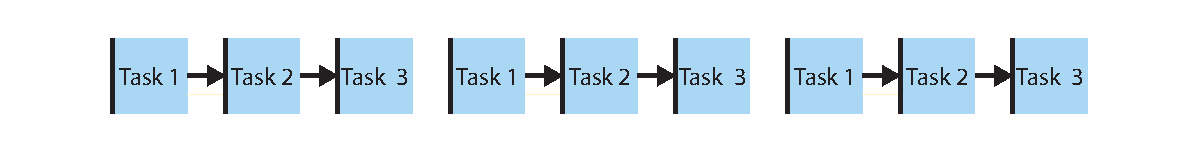
\includegraphics[width=\textwidth]{figures/concurrency/sequential.pdf}
    \caption{Visualisation of a sequential execution.}
    \label{fig:concurrency_sequential}
\end{figure}

\begin{figure}
    \centering
    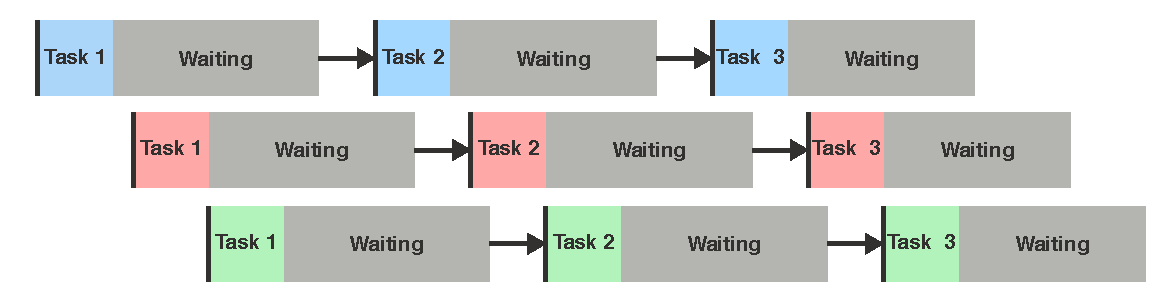
\includegraphics[width=\textwidth]{figures/concurrency/concurrent.pdf}
    \caption{Visualisation of a concurrent execution.}
    \label{fig:concurrency_concurrent}
\end{figure}

\begin{figure}
    \centering
    
\includegraphics[width=\textwidth]{figures/concurrency/paralell.pdf}
    \caption{Visualisation of a parallel execution.}
    \label{fig:concurrency_parallel}
\end{figure}

\subsection{Context switching}

\subsection{Parallel execution}

\subsection{In python}

\subsection{Message passing}
\subsubsection{}
\begin{itemize}
    \item Can the task be done in parallel?
    \item Does the task require a lot of memory?
    \item Does the order of output matter?
    \item Is latency an issue?
    \item Is there any bottlenecks?
    \item What tasks are resource intensive?

\end{itemize}